% Document Type/Class
\documentclass[12pt,a4paper]{article}

% Packages 
\usepackage[utf8]{inputenc}
\usepackage[T1]{fontenc}
\usepackage[spanish]{babel}
\usepackage{epstopdf}
\usepackage{amsmath}
\usepackage{amsfonts}
\usepackage{amssymb}
\usepackage{graphicx}
\usepackage{siunitx}
\usepackage{parskip}
\usepackage{gensymb}
\usepackage{multicol}

\newcommand{\expnum}[2]{{#1}\mathrm{e}{#2}}
\newcommand{\eee}[2]{{#1}\times 10^{#2}}

% Document Options 
\linespread{1.25}
\decimalpoint

\begin{document}
	
	\begin{titlepage}
		\begin{center}
      % Upper margin  
      \vspace{2cm}
      
      % Title -> Large + Bold
      \huge
      \textbf{Diseño de un Controlador por el Método del Lugar de las Raíces}
      
      % Vertical space
      \vspace{.5cm}
      
      % So
      \large
      Proyecto Final
      
      % Vertical Space (Tune)
      \vspace{2cm}

      \small
      \textbf{Zaira Lakeisha Rodríguez González} \break
      \textbf{Kevin Fernando Becerra Núñez} \break
      \textbf{Brandon Olaf Contreras Herrera} \break
      \textbf{Luis Fernando Maravilla Valdivia} \break
      \textbf{Diego Alejandro Sánchez Kelly} \break

      % Vertical space (Tune)
      \vspace{1cm}
      
      % Institution logo
      
\includegraphics[width=0.4\textwidth, keepaspectratio]{./Resources/UDG.png}
      
      % Vertical fill sets the lower margin automatically
      \vfill
      
      % Subject & Institution
      \large
      Ingeniería de Control \break
      Universidad de Guadalajara.

      % Lower margin is automatic
		\end{center}
	\end{titlepage}

  % Mandatory pagebreak
	\pagebreak 
	
    \begin{center}
      \textbf{Abstract} \break
      Utilizando el sistema de demostración IP01/IP02 de la marca Quanser, se diseñó un controlador de posición 
      para una planta que consiste en un carro con masa montado en un eje lineal. El diseño del controlador se llevó 
      por medio del método del luga geométrico de las raíces o LGR. 
    \end{center}

  % Optional pagebreak  
	%\pagebreak
	
    \tableofcontents
	
  % Mandatory pagebreak   
	\pagebreak

	  \section{Introducción} \label{sec:intro}
	
      El diseño del controlador comienza con el modelado matemático de la dinámica del sistema seleccionado. Para 
      facilitar el trabajo, el fabricante se ha encargado de proporcionar un análisis de la dinámica del sistema, 
      a continuación, un resumen del mismo. 

      \subsection{Descripción de la Planta}

        La planta de demostración está compuesta por un carro montado en un eje horizontal de acero, así como un 
        eje secundario que permite estabilizar el movimiento del sistema.

        En el eje secundario, el carrito implementa un par de engranajes, que alimentan a un encoder rotatorio de 
        cuadratura o un potenciómetro analógico, según el modelo del dispositivo. 

        El dispositivo, entonces, permite conocer la posición del carrito por medio de 2 diferentes mecanismos, 
        por extensión, esto también permite conocer la velocidad y aceleración del mismo. La Figura~\ref{fig:intro:planta}
        muestra el dispositivo, cortesía del fabricante.

        \vfill

        \begin{figure}[h]
          \centering
          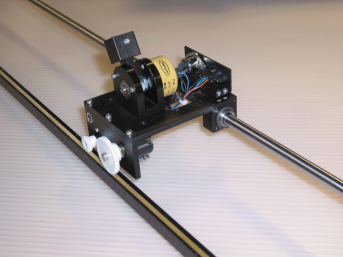
\includegraphics[width=0.65\textwidth, keepaspectratio]{./Resources/IP01.png}
          \caption{Planta}
          \label{fig:intro:planta}
        \end{figure}

    \pagebreak

	  \section{Modelado}

      El modelado del dispositivo en su mayoría es realizado por el fabricante en el manual de usuario, por lo que 
      a continuación se presenta un resumen de los cálculos a partir de los cuales se derivan las funciones de 
      transferencia de lazo abierto y lazo cerrado. 

      \subsection{Lazo Abierto}  

        \subsubsection{Función de Transferencia}

        El fabricante obtiene 2 modelos matemáticos de la dinámica del sistema, por un lado, un modelo simplificado, 
        como ejercicio, y posteriormente un modelo más completo, óptimo para el diseño de un controlador. 
        
        La función de transferencia de lazo abierto para el modelo complejo es la siguiente, 
        
        \begin{equation}
          G\left(s\right) = \frac{r_{mp} \eta_{g} K_{g} \eta_{m} K_{t}}{s^{2}\left(R_{m} M r_{mp}^{2} \eta_{g} K_{g}^{2} J_{m}\right) + 
          s\left(\eta_{g} K_{g}^{2} \eta_{m} K_{t} K_{m} + B_{eq} R_{m} r_{mp}^{2}\right)}
          \label{eq:modeling:plantTf}
        \end{equation}

        La sustitución de los parámetros físicos de la planta en la Ecuación~\ref{eq:modeling:plantTf} produce la
        siguiente función, 
        
        \begin{equation}
          G\left(s\right) = \frac{\expnum{1.8063}{-4}}{s^{2}\left(\expnum{6.8472}{-5}\right) + s\left(\expnum{1.2605}{-3}\right)}
          \label{eq:modeling:openLoopTf_nosimp}
        \end{equation}

        Esto se puede simplificar posteriormente, tal que,  
        
        \begin{equation}
          G\left(s\right) = \frac{2.638}{s^{2} + s\left(18.409\right)}
          \label{eq:modeling:openloopTf_simpd}
        \end{equation}

        La anterior operación no modifica la ubicación de los polos y ceros del controlador, sin embargo, 
        si permite que los cálculos posteriores sean más sencillos. 

        \subsubsection{Polos y Ceros}

        La retroalimentación negativa no altera las propiedades de los polos y ceros del sistema, asimismo, no 
        incrementa o reduce su cantidad. Por lo tanto, el análisis de su ubicación se puede realizar antes o después de
        aplicar retroalimentación negativa. 

        De la función de transferencia de lazo abierto, se obtiene

          \begin{equation*}
            \begin{aligned}
              s^{2}+ s\left(18.4092\right) &= 0 \\
              s^{2} &= -s\left(18.4092\right)\\
            \end{aligned}
            \label{eq*:modeling:roots}
          \end{equation*}    

          de lo anterior, \(s \rightarrow \left\{0, -18.4092\right\}\) en el caso de los polos. 

          Asimismo, observando el numerador de la función original, es evidente que no existen ceros. 

          Es posible verificar la ubicación de los polos y ceros en la Figura~\ref{fig:modeling:pzmap_open}

          \begin{figure}
            \centering
            \includegraphics[width=0.75\textwidth, keepaspectratio]{./Resources/pzmap_ol.png}
            \caption{Mapa de polos y ceros, Lazo Abierto}
            \label{fig:modeling:pzmap_open}
          \end{figure}

      \subsection{Lazo Cerrado}    
      
        Se aplica una retroalimentación negativa a la función de transferencia de la Ecuación~\ref{eq:modeling:openloopTf_simpd}.

        Esto se realiza por medio del comando \verb|feedback(tf, 1, -1)|, el cual genera un lazo cerrado con ganancia 
        unitaria negativa. 

        La función de transferencia de lazo cerrado, entonces,

        \begin{equation}
          G\left(s\right) = \frac{2.638}{s^{2} + s\left(18.4092\right) + 2.638}
          \label{eq:model:closedLoopTf}
        \end{equation}

      \subsubsection{Polos y Ceros}
        	
        Por consistencia, comprobamos la locación de los polos y ceros del sistema, que no deben modificarse
        debido a la retroalimentación aplicada al sistema.

        Por lo tanto, lo establecido en la Sección~\ref{eq*:modeling:roots} debe mantenerse, y, como se puede ver en la 
        Figura~\ref{fig:modeling:pzmap_closed}, el lugar geométrico de las raíces no se modifica. 

        \begin{figure}
          \centering
          \includegraphics[width=0.75\textwidth, keepaspectratio]{./Resources/pzmap_cl_nc.png}
          \caption{Mapa de Polos y Ceros, Lazo Cerrado.}
          \label{fig:modeling:pzmap_closed}
        \end{figure}

    \pagebreak

    \section{Análisis de Respuesta en el Tiempo}

    Previo a comenzar el diseño del controlador, es necesario conocer la respuesta del sistema a diferentes 
    estímulos o perturbaciones. Esto es relevante ya que nos permitirá determinar el tipo de controlador 
    y sus parámetros de diseño. 

    El diseño contempla el uso del lugar geométrico de las raíces para diseñar un compensador de adelanto, por lo 
    tanto, el análisis de la respuesta se realiza en el dominio del tiempo y no de la frecuencia. 

    Entonces, el primer paso es conocer la respuesta transitoria del sistema, comenzando por la respuesta 
    a una función escalón. 

    \subsection{Escalón Unitario}
      
      Utilizando el comando \verb|step| en MATLAB, es posible obtener la respuesta en el tiempo del sistema 
      a un estímulo escalón.   

      La Figura~\ref{fig:response:closedLoopStep} muestra la respuesta en lazo cerrado del sistema a un 
      estímulo constante de amplitud 1. Esta respuesta es característica de un sistema de segundo orden

      Como puede observarse, la respuesta del sistema es lenta. Extrayendo los valores de la misma gráfica, 
      el tiempo de subida es de \(15.2\si{\second}\), mientras que el tiempo de asentamiento es 
      de \(27.1\si{\second}\).

      \begin{figure}
        \centering
        \includegraphics[width=0.75\textwidth, keepaspectratio]{./Resources/cltf_step_nc.png}
        \caption{Respuesta Escalón Unitario, Lazo Cerrado}
        \label{fig:response:closedLoopStep}
      \end{figure}

  \pagebreak

  \section{Diseño del Compensador}

      Un compensador de adelanto tiene la intención de cambiar la respuesta del sistema introduciendo un polo y un cero. Esto 
      tiene el efecto de mover el LGR para hacerlos pasar por una serie de polos deseados. 

      Posteriormente, se sintoniza el controlador seleccionando la ganancia adecuada para la cuál la condición de ángulo 
      se cumple. 

      Los compensadores, ya sean de adelanto, retardo o adelanto-retardo, no son controladores propiamente, sin embargo, permiten
      implementar acciones de control de forma mucho más sencilla que, por ejemplo, un controlador PID. 

      A continuación se proporciona contexto sobre el proceso, fórmulas y técnicas de diseño utilizadas para 
      el diseño final del controlador.

      \subsection{Marco Teórico}

        La teoría de control proporciona una serie de herramientas para moldear la respuesta de un sistema según 
        lo requerido por el diseñador. 

        Para un sistema de segundo orden, (ver Ecuación~\ref{eq:model:closedLoopTf}), la forma normal del sistema 
        tiene las siguiente ecuación estándar, 

        \begin{equation}
          G\left(s\right) = \frac{K_{dc}\omega_{n}^{2}}{s^{2} + 2\zeta\omega_{n}s + \omega_{n}^{2}}
          \label{eq:design:2ndorder_std}
        \end{equation}

        con polinomio característico, 

        \begin{equation}
          s^{2} + 2\zeta\omega_{n}s + \omega_{n}^{2}
          \label{eq:design:2ndorder_std_charact}
        \end{equation}

        También sabemos que los parámetros de sobredisparo y tiempo pico se pueden calcular con las siguientes ecuaciones, 
        respectivamente, 

        \begin{equation}
          P_{osht} = 100\exp\left(-\frac{\zeta\pi}{\sqrt[2]{1-\zeta^{2}}}\right)
          \label{eq:design:overshoot_prcntg}
        \end{equation}

        \begin{equation}
          t_{p} = \frac{\pi}{\omega_{n}\sqrt{1-\zeta^{2}}}
          \label{eq:design:peak_time}
        \end{equation}

      \subsection{Parámetros de diseño}

        Se proponen los siguientes parámetros de diseño,

        \begin{description}
          \item[Overshoot] El sistema debe contar con un porcentaje de sobredisparo de máximo un 7\%. 
          \item[Peak Time] El sistema debe alcanzar su punto pico en $ 110\si{\milli\second} $. 
        \end{description}
      
      \subsection{Ubicación de los Polos Deseados}

        Desde \ref{eq:design:overshoot_prcntg}, 

        \begin{equation}
        \zeta = \frac{-\ln\left(P_{osht}\right)}{\sqrt{\pi^{2} + \ln^{2}\left(P_{ovsht}\right)}}
        \end{equation}

        y, desde, \ref{eq:design:peak_time}, 

        \begin{equation}
          \omega_{n} = \frac{\pi}{t_{p}\sqrt{1-\zeta^{2}}}
        \end{equation}
        
        entonces, calculando los valores de $ \zeta $ y de $ \omega_{n} $, obtenemos, 

        \begin{equation*}
          \begin{aligned}
            \zeta &= \frac{-\ln\left(0.08\right)}{\sqrt{\pi^{2} + \ln^{2}\left(0.08\right)}} \\
            \zeta &= 0.64608 \\
          \end{aligned}
        \end{equation*}

        y, 

        \begin{equation*}
          \begin{aligned}
            \omega_{n} &= \frac{\pi}{0.11\sqrt{1-\zeta^{2}}} \\ 
            \omega_{n} &= 37.42218 \\
          \end{aligned}
        \end{equation*}
        
        Despejando $ S $ en la Ecuación~\ref{eq:design:2ndorder_std_charact}, se obtiene que, 

        \begin{equation}
          s = -\zeta\omega_{n} \pm \omega_{n}\sqrt{1 - \zeta^{2}}j
          \label{eq:design:charact_sval}
        \end{equation}

        y, posteriormente, sustituyendo los valores de $ \zeta $ y de $ \omega_{n} $ calculados anteriormente, 
        obtenemos,

        \begin{equation}
          \centering
          \begin{aligned}
            \hat{s} &= \left(-0.64608\right) \left(37.42218\right) \pm \left(37.42218\sqrt{1-0.64608^{2}}\right) \\
            \hat{s} &= -24.17772 \pm 32.69379j
          \end{aligned}
        \end{equation}

        Que es la combinación compleja conjugada de los polos deseados para el compensador de adelanto. 

      \subsection{Condición de Ángulo}

        Conociendo la ubiación deseada del polo, el primer paso es entonces verificar si este ya se encuentra en 
        el lugar geométrico de las raíces, lo cual requiere de aplicar la condición de ángulo. 

        La condición de ángulo establece que, 

        \begin{equation}
          \Sigma_{\angle_{poles}} + \Sigma_{\angle_{zeros}} = 180\degree
          \label{eq:design:angle_condition} 
        \end{equation}

        Calculando,
        
        \[ \alpha_{1} = 180\degree - tan^{-1}\left(\dfrac{32.69379}{24.17772}\right) \]

        y 

        \[ \alpha_{2} = 180\degree - tan^{-1}\left(\dfrac{32.69379}{24.17772 - 18.40923}\right) \]

        lo cual resulta en \( \alpha_{1} = 126.48367\degree \) y \( \alpha_{2} = 100.00627 \).

        Podemos calcular el ángulo de deficiencias, 

        \begin{equation}
          \phi = 180\degree - \alpha_{1} - \alpha_{2} 
        \end{equation}

        entonces, 

        \[ \phi =  180\degree - 126.48367\degree - 100.00627\degree \]

        por lo tanto, \( \phi = 46.48994\degree \).

        Este ángulo, \( \phi \), corresponde al ángulo que deberá proporcionar el compensador para lograr que 
        el lugar geométrico de las raíces pase por el polo deseado. 

      \subsection{Polos y ceros del compensador}
        \label{subsec:polezero}

        Calulamos la sintonización, 

        \[ \dfrac{\phi}{2} = 23.24497\degree \]

        por lo tanto, 

        \[ \alpha_{3} = \dfrac{\alpha_{1}}{2} = \dfrac{126.48367}{2}  \]

        que es, \( \alpha_{3} = 63.2418 \). También, 

        \[ \alpha_{4} = \alpha_{3} - \dfrac{\phi}{2} = 63.2418 - \dfrac{46.4894}{2} \], 
        
        que es \( 39.9968 \). 

        Entonces, 

        \[ \tan\left(39.9968\right)\dfrac{32.6937}{d} \]

        Calculando \( d \), 

        \[ d = \dfrac{32.6937}{\tan\left(39.9968\right)} = 38.9672 \]

        A partir de lo anterior, es posible calcular el polo compensado, 
        
        \[ \dfrac{1}{\alpha } = 38.9672 + 24.1777 = 69.1449 \]

        similarmente, podemos calcular el cero compensado, 

        \[ \tan\left(3.5131 \right) = \dfrac{y}{32.69379} \]

        despejando, 

        \[ y = 32.6937 \cdot \tan\left(3.5131\right) = 2.0071 \]

        Finalmente, 

        \[ \dfrac{1}{T} = 24.1777 + 2.0071 = 26.1849\]

        A partir de esto, es posible proceder con la implementación del controlador y la obtención de la función 
        de transferencia final. 

	\pagebreak
	
	\section{Desarrollo del Compensador de Adelanto}
	
    La forma estándar de un compensador de adelanto es la siguiente, 

    \begin{equation}  
      G_{c}\left(s\right) = K_{c}\dfrac{s+\dfrac{1}{T}}{s + \dfrac{1}{\alpha T}}
      \label{eq:devel:leadcomp}
    \end{equation}

    donde \( \alpha \) debe encontrarse en la región \( 0 < \alpha < 1 \). 

    Según lo establecido en la Sección~\ref{subsec:polezero}, sustituímos en la 
    Ecuación~\ref{eq:devel:leadcomp} para obtener, 

    \[ G_{c}\left(s\right) = K_{c}\dfrac{s + 26.18491}{s + 63.1449}\]
        
    \subsection{Ganancia del Compensador}

      Desde, 

      \begin{equation}
        0 = 1 + G_{c}\left(s\right)G\left(s\right)
        \label{eq:devel:compdsys_formula}
      \end{equation}

      sustituímos, 

      \[ 1 + K_{c}\left(\dfrac{s + 26.1849}{s + 63.1449}\right)\left(\dfrac{2.6389}{s\left(s + 18.4092\right)}\right) = 0 \]

      y, posteriormente, evaluamos en \( \hat{s} \), 

      \[ K_{c}\left|\left(\dfrac{s + 26.1849}{s + 63.1449}\right)\left(\dfrac{2.6389}{s\left(s + 18.4092\right)}\right)\right| = 1 \]

      tal que, 

      \[ K_{c} = 794.39503 \]

      Al proceso anterior se le conoce como la \emph{condición de magnitud}. 

    \subsection{Función de Transferencia Compensada} 

      Finalmente, 

      \begin{equation*}
        G_{c}\left(s\right)G_{s}\left(s\right) = 794.39503\frac{2.63891s + 69.0996}{s^{3} + 81.5542s^{2} + 1162.45s}
      \end{equation*}

      Que es el sistema final compensado. 

  \pagebreak

  \section{Análisis del Controlador}

    Una vez obtenida la función de transferencia de la planta en serie con el controlador, en serie, es posible determinar 
    la respuesta del sistema completo y verificar que se ha modificado a la respuesta deseada. 

    Para ello, es de nuestro interés comparar las respuestas a los posibles estímulos al sistema, 

    

\end{document}